\documentclass[10pt]{beamer}
% \usetheme{Boadilla}
  \usetheme{default}


% acronyms for text or math mode
\newcommand {\ccast} {\mbox{\small\textsc{ccast}}}
\newcommand {\kcarta} {\mbox{k\small{CARTA}}}

\newcommand {\cris} {\mbox{\small CrIS}}
\newcommand {\airs} {\mbox{\small AIRS}}
\newcommand {\iasi} {\mbox{\small IASI}}
\newcommand {\idps} {\mbox{\small IDPS}}
\newcommand {\nasa} {\mbox{\small NASA}}
\newcommand {\noaa} {\mbox{\small NOAA}}
\newcommand {\nstar} {\mbox{\small STAR}}
\newcommand {\umbc} {\mbox{\small UMBC}}
\newcommand {\uw}   {\mbox{\small UW}}

\newcommand {\fft}  {\mbox{\small FFT}}
\newcommand {\ifft} {\mbox{\small IFFT}}
\newcommand {\fir}  {\mbox{\small FIR}}
\newcommand {\fov}  {\mbox{\small FOV}}
\newcommand {\for}  {\mbox{\small FOR}}
\newcommand {\ict}  {\mbox{\small ICT}}
\newcommand {\ils}  {\mbox{\small ILS}}
\newcommand {\igm}  {\mbox{\small IGM}}
\newcommand {\opd}  {\mbox{\small OPD}}
\newcommand {\rms}  {\mbox{\small RMS}}
\newcommand {\zpd}  {\mbox{\small ZPD}}
\newcommand {\ppm}  {\mbox{\small PPM}}
\newcommand {\srf}  {\mbox{\small SRF}}
\newcommand {\sdr}  {\mbox{\small SDR}}
\newcommand {\FWHM} {\mbox{\small FWHM}}
\newcommand {\fwhm} {\mbox{\small\textsc{fwhm}}}

\newcommand {\ES} {\mbox{\small ES}}
\newcommand {\SP} {\mbox{\small SP}}
\newcommand {\IT} {\mbox{\small IT}}
\newcommand {\SA} {\mbox{\small SA}}

\newcommand {\ET} {\mbox{\small ET}}
\newcommand {\FT} {\mbox{\small FT}}

\newcommand {\wn} {\mbox{cm$^{-1}$}}
\newcommand {\cm} {\mbox{cm}}

% abbreviations, mainly for math mode
\newcommand {\real} {\mbox{real}}
\newcommand {\imag} {\mbox{imag}}
\newcommand {\atan} {\mbox{atan}}
\newcommand {\obs}  {\mbox{obs}}
\newcommand {\calc} {\mbox{calc}}
\newcommand {\sinc} {\mbox{sinc}}
\newcommand {\psinc} {\mbox{psinc}}
\newcommand {\std} {\mbox{std}}

% symbols, for math mode only
\newcommand {\lmax} {L_{\mbox{\tiny max}}}
\newcommand {\vmax} {V_{\mbox{\tiny max}}}

\newcommand {\tauobs} {\tau_{\mbox{\tiny obs}}}
\newcommand {\taucal} {\tau_{\mbox{\tiny calc}}}
\newcommand {\Vdc}  {V_{\mbox{\tiny DC}}}

\newcommand {\rIT} {r_{\mbox{\tiny\textsc{ict}}}}
\newcommand {\rES} {r_{\mbox{\tiny\textsc{es}}}}
\newcommand {\robs} {r_{\mbox{\tiny obs}}}

\newcommand {\rITobs} {r_{\mbox{\tiny\textsc{ict}}}^{\mbox{\tiny obs}}}
\newcommand {\rITcal} {r_{\mbox{\tiny\textsc{ict}}}^{\mbox{\tiny cal}}}

\newcommand {\rESuser} {r_{\mbox{\tiny\textsc{es}}}^{\mbox{\tiny user}}}
\newcommand {\rITuser} {r_{\mbox{\tiny\textsc{ict}}}^{\mbox{\tiny user}}}
\newcommand {\rITsensor} {r_{\mbox{\tiny\textsc{ict}}}^{\mbox{\tiny sensor}}}
\newcommand {\rITfov} {r_{\mbox{\tiny\textsc{ict}}}^{\mbox{\tiny fov}}}

\newcommand {\fcos} {f_{\mbox{\tiny cos}}}
\newcommand {\fatbd} {f_{\mbox{\tiny\textsc{atbd}}}}

\newcommand {\ITmean} {\langle\mbox{\small IT}\rangle}
\newcommand {\SPmean} {\langle\mbox{\small SP}\rangle}

\newcommand {\Ttc} {t^{\mbox{\tiny\textsc{tc}}}}
\newcommand {\Tac} {t^{\mbox{\tiny\textsc{ac}}}}
\newcommand {\rtc} {r_{\mbox{\tiny\textsc{tc}}}}
\newcommand {\rta} {r_{\mbox{\tiny\textsc{ta}}}}



\title{A first look at the Jan 2020\\
  CrIS TVAC PFL gas cell tests}
\author{H.~E.~Motteler, L.~L.~Strow, \\
  S.~DeSouza-Machado, \\
  S.~Buczkowski
}
\institute{
  UMBC Atmospheric Spectroscopy Lab \\
  Joint Center for Earth Systems Technology \\
}
\date{\today}
\begin{document}

%----------- slide --------------------------------------------------%
\begin{frame}[plain]
\titlepage
\end{frame}
%----------- slide --------------------------------------------------%
\begin{frame}
\frametitle{Introduction}
\begin{itemize}

\item We present an analysis of the PFL Plateau 20 CH$_4$, CO$_2$,
  and CO gas cell tests, and compare these with calculated reference
  truth from LBLRTM and UMBC-LBL.

  \item This is a reanalysis with more careful harvesting of the
    individual test legs and better calculated transmittances.  The
    resulting changes to the metrology laser relative residuals were
    less than 1 ppm.
 
   \item Examples of monitoring test logs (the CSS, CMD, and TCR
     files) are given in the form of plots of HTBB temperature, gas
     cell temperature, and gas cell pressure over time.

  \item The J2 tests continue to be done at the older 866/1052/799
    point resolutions.
    
\end{itemize}
\end{frame}
%----------- slide --------------------------------------------------%
\begin{frame}
\frametitle{Methods}
\begin{itemize}

  \item For each gas we partition the data stream into four test
    legs, \\ FT1, FT2, ET1, and ET2 (cell full, HTBB temperature T1,
    etc.)

  \item For test each leg, we take the mean of the associated count
    spectra, calculate the transmittance as $(FT2 - FT1) / (ET2 -
    ET1)$, apply our standard processing filters, and do the SA
    correction, all at the sensor grid.  Expected transmittance
    values are also calculated at the sensor grid.

  \item This is similar in some ways to the ``ratio first''
    calibration algorithm used as an option in UMBC CCAST
    processing, but note that we do not do a full radiance
    calibration, or any nonlinearity correction, for the analysis
    here.

  \item Measured and calculated transmittances are compared first as
    is, and then by fitting obs to calcs and examining fitting
    weights and residuals.

  \item This approach, with fitting adjustments, is acceptable for
    our application because our main task is spectral calibration
    and our fitting methods are robust in the face of radiometric
    uncertainty.

\end{itemize}
\end{frame}
%----------- slide --------------------------------------------------%
\begin{frame}
\frametitle{7-8 Jan 2020 TVAC PFL Plateau 20}
\begin{columns}[t]
\begin{column}{0.5\textwidth}
  \begin{centering}
  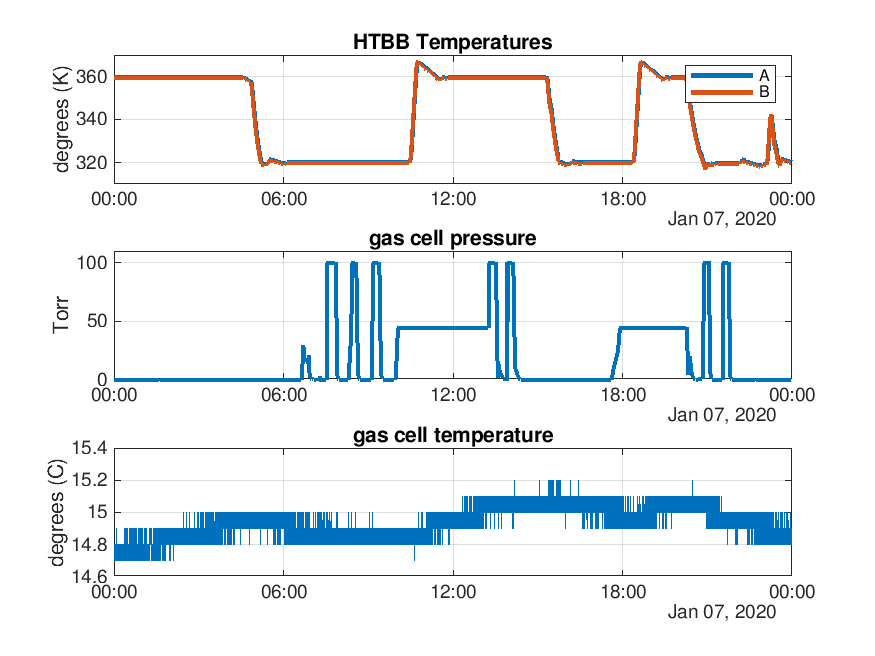
\includegraphics[width=\textwidth]{harvest_01-07/css_summary_07_jan.png}
  \end{centering}\vspace{3mm}

\end{column}
\begin{column}{0.5\textwidth}  
  \begin{centering}
  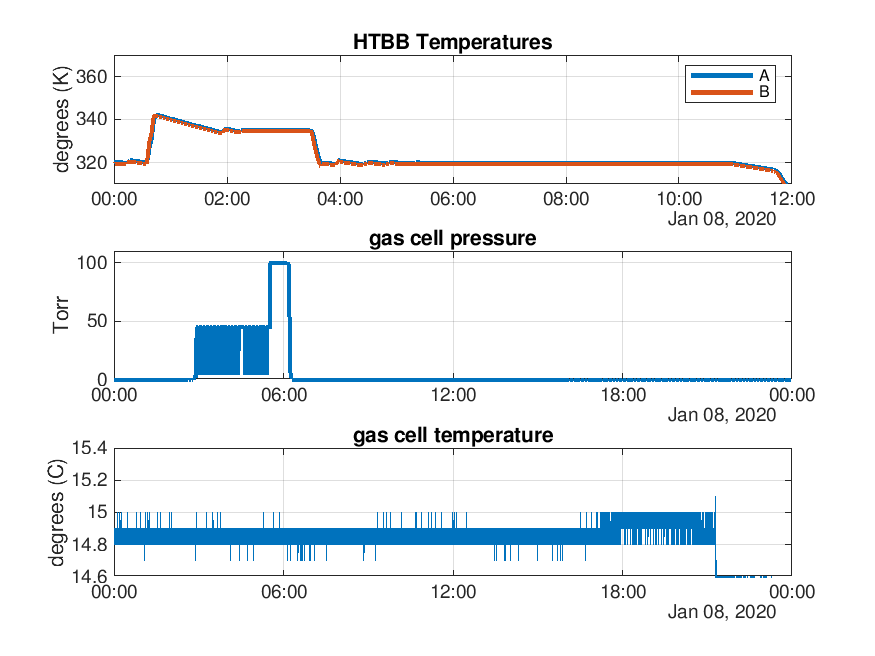
\includegraphics[width=\textwidth]{harvest_01-07/css_summary_08_jan.png}
  \end{centering}\vspace{3mm}

\end{column}
\end{columns}

HTBB temperatures, gas cell pressure and gas cell temperature from
the CCS files, for 7-8 Jan 2020.  This data is used along with a
scan of the CMD and SQL files for an overview and to find the test
stages.

\end{frame}
%----------- slide --------------------------------------------------%
\begin{frame}
\frametitle{CH$_4$ MW PFL side 1 test parameters}

\begin{itemize}
  \item PFL Plateau 20, 7-8 Jan 2019
  \item side 1, sweep direction 0
  \item fitting interval 1220 to 1380 $\wn$
  \item metrology laser 771.97035 nm, from neon 703.44765 nm
  \item ATBD default focal plane
  \item SA correction from ILS with periodic sinc at the sensor grid
  \item HTBB nominal T1 360 K, T2 320 K
  \item gas cell pressure 44.64 torr
  \item gas cell temperature 14.90 C
  \item gas cell length 12.59 cm
\end{itemize}

\end{frame}
%----------- slide --------------------------------------------------%
\begin{frame}
\frametitle{CH$_4$ PFL side 1 cell empty test legs}
\begin{columns}[t]
\begin{column}{0.5\textwidth}
  \begin{centering}
  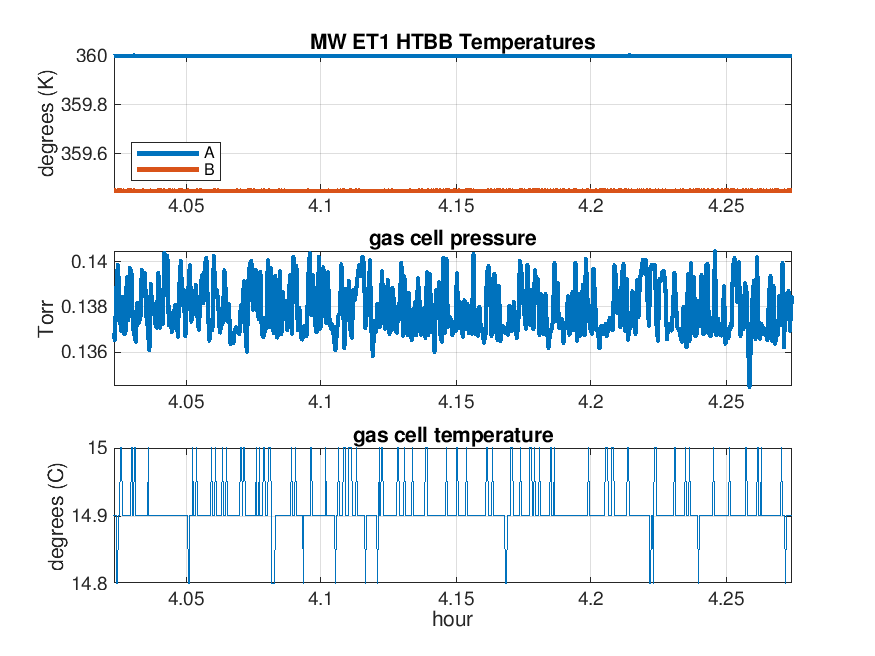
\includegraphics[width=\textwidth]{harvest_01-07/01-07_MW_ET1.png}
  \end{centering}\vspace{3mm}

  ET1 ``empty high'' leg of the the 7 Jan CH$_4$ transmittance test.
  The x-axis is hour of the day.  This looks good.

\end{column}
\begin{column}{0.5\textwidth}  
  \begin{centering}
  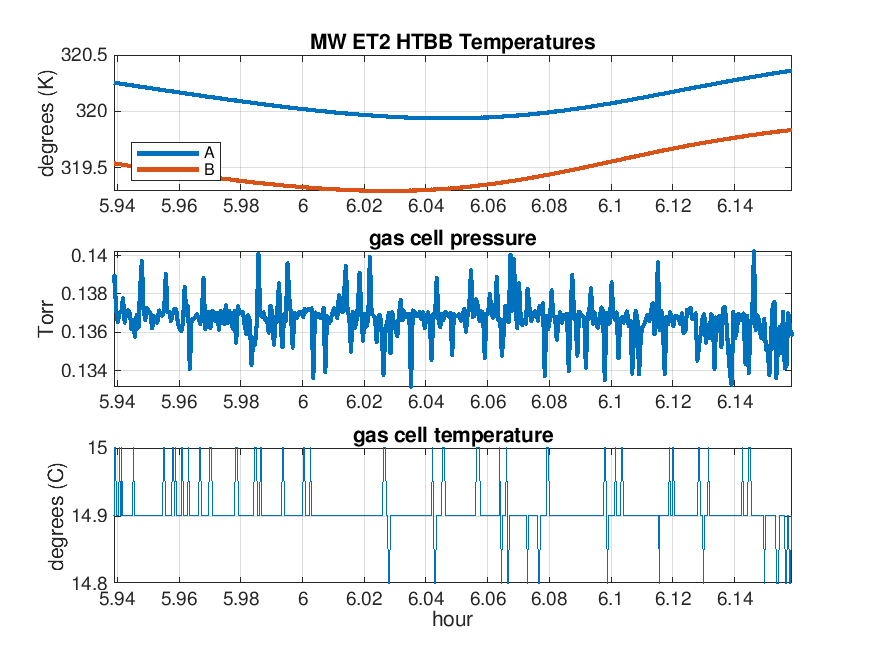
\includegraphics[width=\textwidth]{harvest_01-07/01-07_MW_ET2.png}
  \end{centering}\vspace{3mm}

  ET2 ``empty low'' leg of the the 7 Jan CH$_4$ transmittance test.
  We see some HTBB drift.

\end{column}
\end{columns}
\end{frame}
%----------- slide --------------------------------------------------%
\begin{frame}
\frametitle{CH$_4$ PFL side 1 cell full test legs}
\begin{columns}[t]
\begin{column}{0.5\textwidth}
  \begin{centering}
  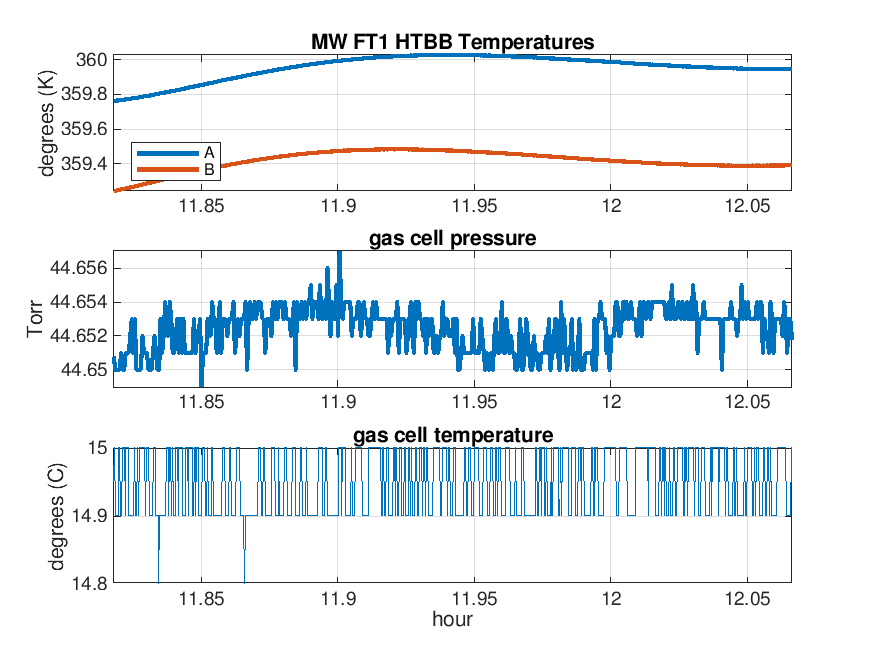
\includegraphics[width=\textwidth]{harvest_01-07/01-07_MW_FT1.png}
  \end{centering}\vspace{3mm}

  FT1 ``full high'' leg of the the 7 Jan CH$_4$ transmittance test.
  The x-axis is hour of the day.  As in the empty low leg we see
  some HTBB drift.

\end{column}
\begin{column}{0.5\textwidth}  
  \begin{centering}
  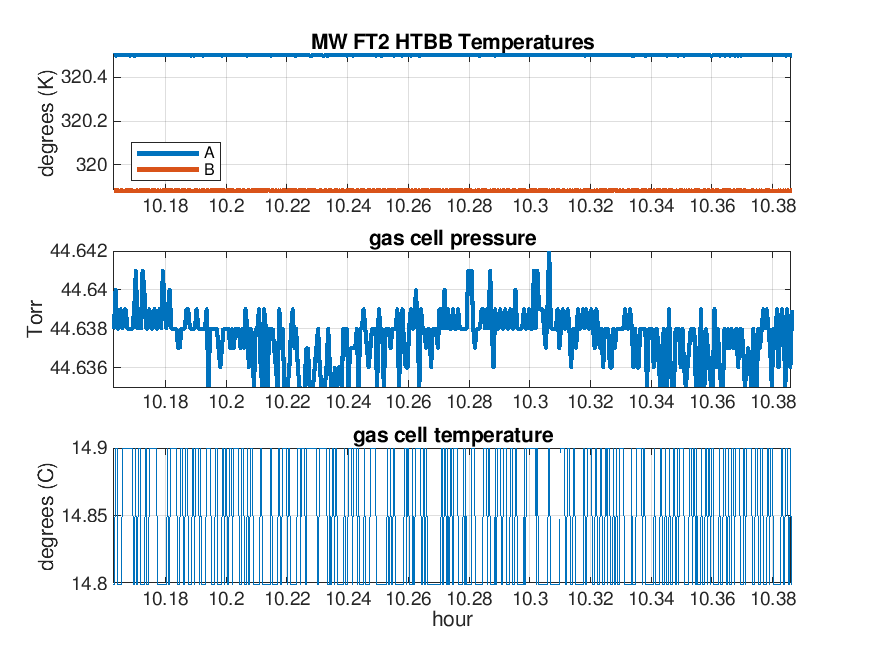
\includegraphics[width=\textwidth]{harvest_01-07/01-07_MW_FT2.png}
  \end{centering}\vspace{3mm}

  FT2 ``full low'' leg of the the 7 Jan CH$_4$ transmittance test.
  This looks good.

\end{column}
\end{columns}
\end{frame}
%----------- slide --------------------------------------------------%
\begin{frame}
\frametitle{CH$_4$ side 1 data before fitting}
\begin{columns}[t]
\begin{column}{0.5\textwidth}  
  \begin{centering}
  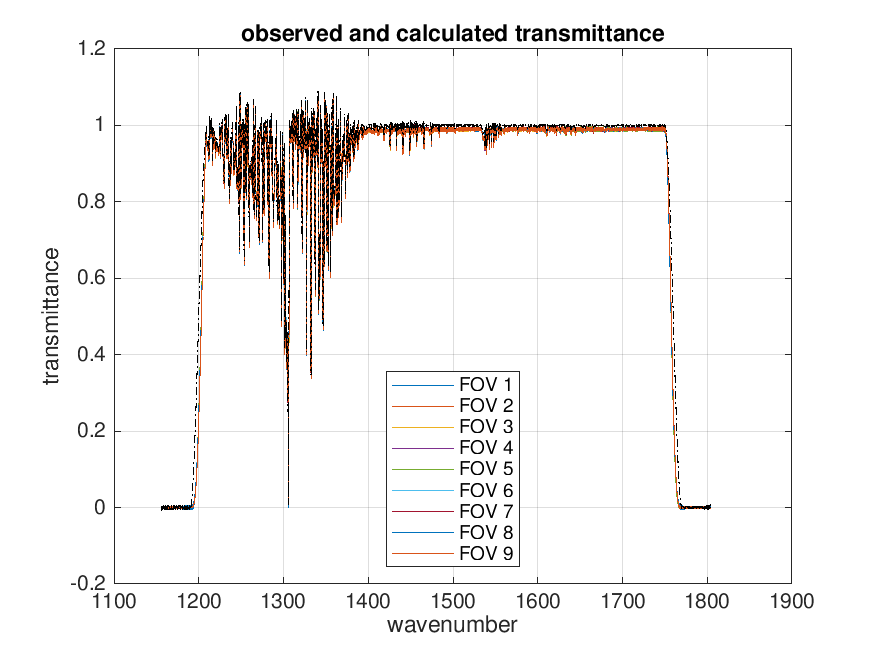
\includegraphics[width=\textwidth]{01-07_pfl_s1_CH4/spec_test2_all.png}
  \end{centering}\vspace{3mm}

Observed and calculated transmittance after the SA correction but
before fitting.  We see some bias in the observed data, possibly due
to problems with the HTBB stability.

\end{column}

\begin{column}{0.5\textwidth}
  \begin{centering}
  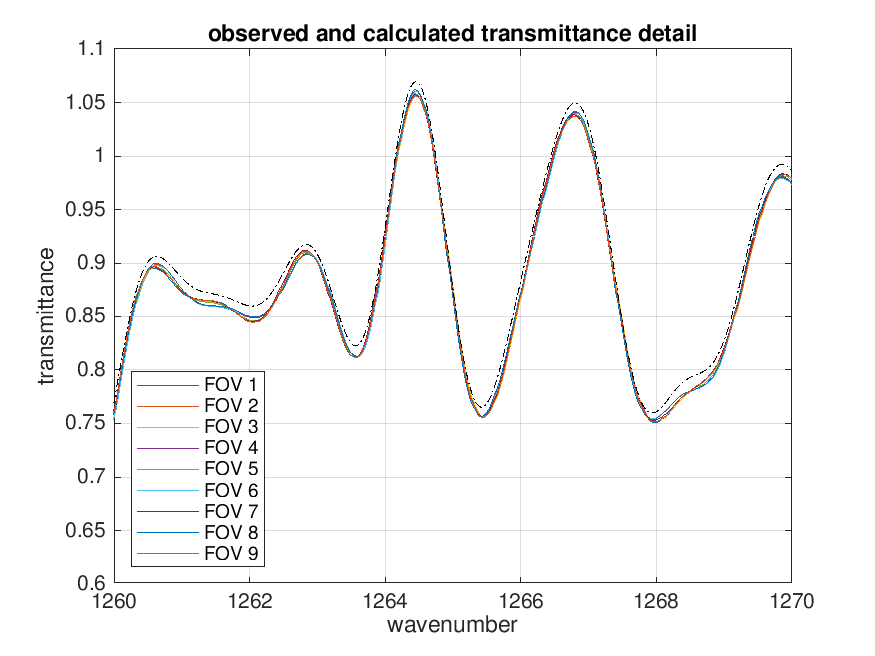
\includegraphics[width=\textwidth]{01-07_pfl_s1_CH4/spec_test2_zoom.png}
  \end{centering}\vspace{3mm}

A detail from the previous plot. Despite the bias, the FOV to FOV
consistency of the observed data is relatively good.

\end{column}
\end{columns}
\end{frame}
%----------- slide --------------------------------------------------%
\begin{frame}
\frametitle{CH$_4$  side 1 fitting overview}
\begin{columns}[t]
\begin{column}{0.5\textwidth}  
  \begin{centering}
  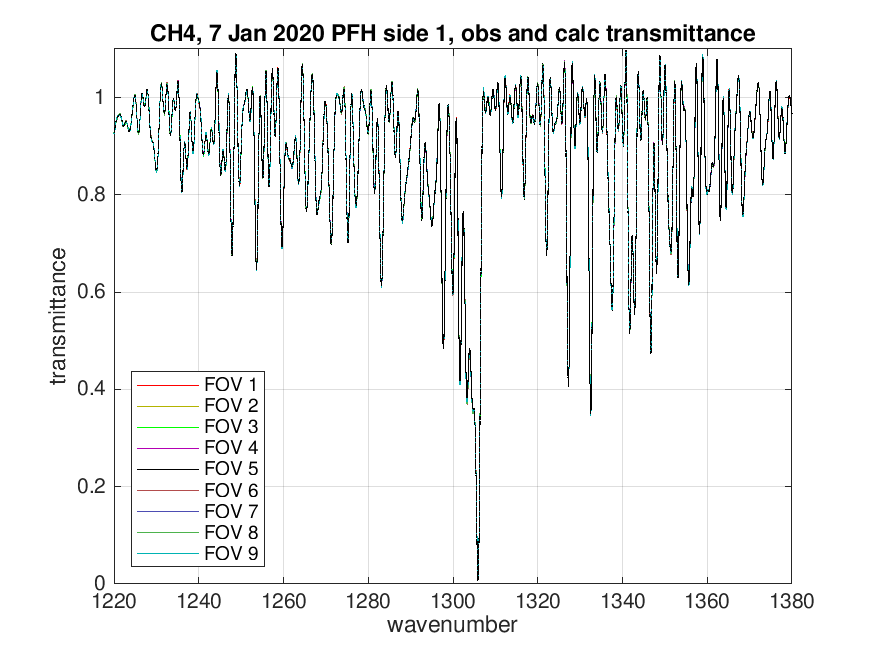
\includegraphics[width=\textwidth]{01-07_pfl_s1_CH4/CH4_obs_and_calc.png}
  \end{centering}\vspace{3mm}

Observed and calculated transmittance for all FOVs, over the fitting
interval.  At this level of detail we see all values are very close.

\end{column}

\begin{column}{0.5\textwidth}
  \begin{centering}
  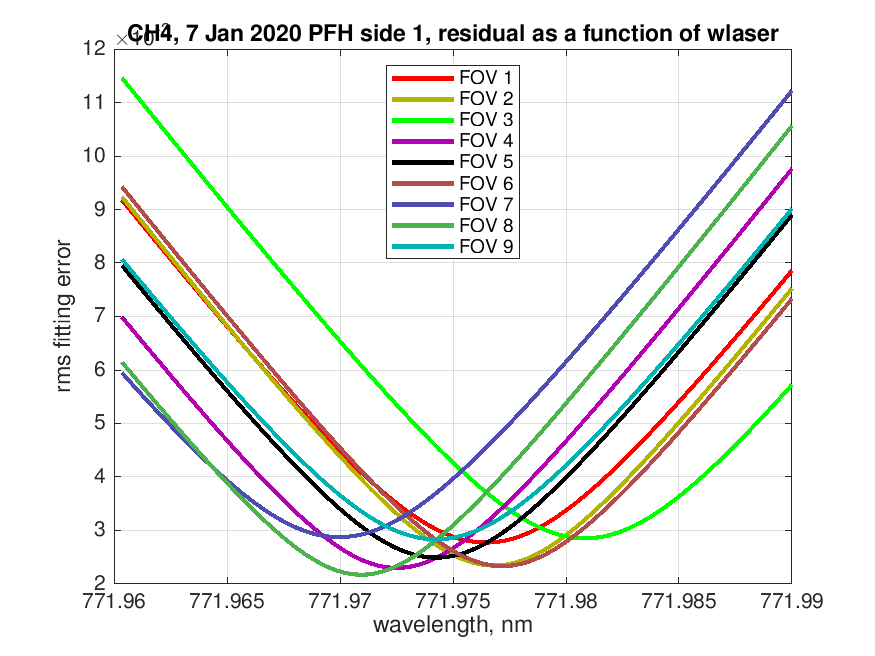
\includegraphics[width=\textwidth]{01-07_pfl_s1_CH4/CH4_wlaser_fit.png}
  \end{centering}\vspace{3mm}

Residuals $\rms(a\cdot\tauobs + b - \taucal)$ over the fitting
interval as a function of metrology laser wavelength, for each FOV.

\end{column}
\end{columns}
\end{frame}
%----------- slide --------------------------------------------------%
\begin{frame}
\frametitle{CH$_4$ side 1 obs minus calc breakouts}
\begin{columns}[t]
\begin{column}{0.5\textwidth}
  \begin{centering}
  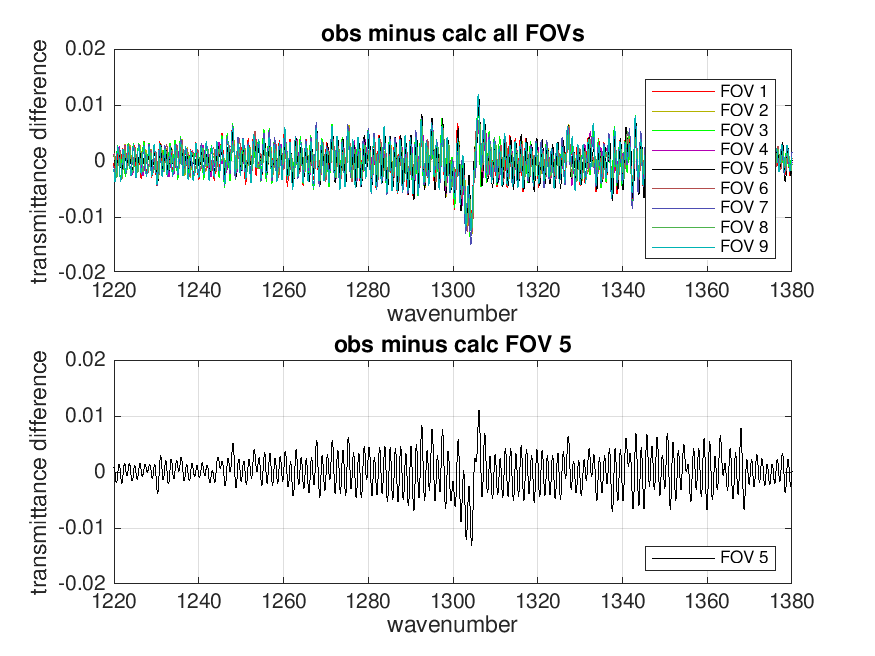
\includegraphics[width=\textwidth]{01-07_pfl_s1_CH4/CH4_breakout_1.png}
  \end{centering}\vspace{3mm}

Observed minus calculated transmittance for all FOVs and for FOV~5
alone, over the fitting interval.

\end{column}
\begin{column}{0.5\textwidth}  
  \begin{centering}
  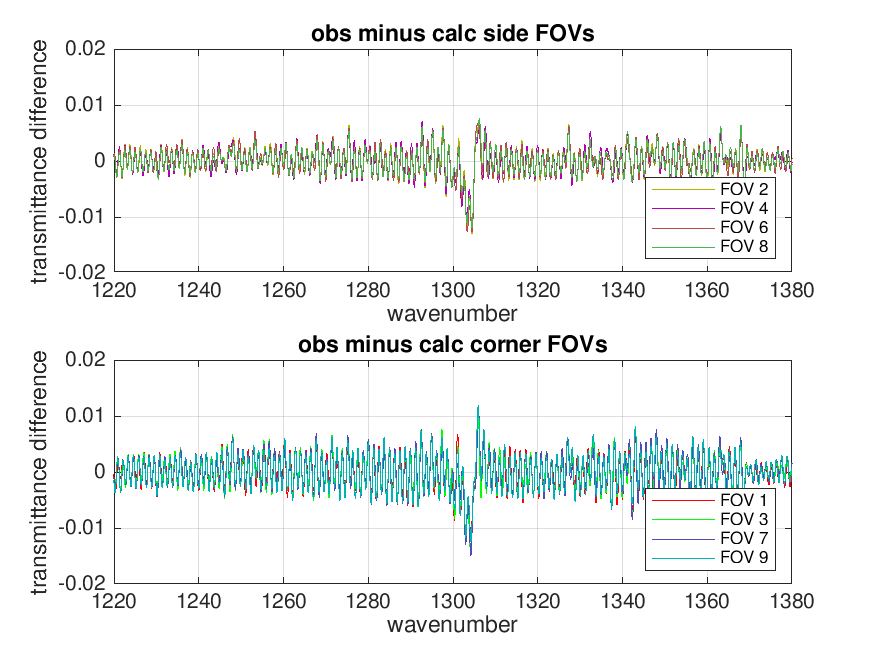
\includegraphics[width=\textwidth]{01-07_pfl_s1_CH4/CH4_breakout_2.png}
  \end{centering}\vspace{3mm}

Observed minus calculated transmittance for side and corner FOVs,
over the fitting interval.

\end{column}
\end{columns}
\end{frame}
%----------- slide --------------------------------------------------%
\begin{frame}[fragile]
\frametitle{CH$_4$ side 1 tabulated residuals}

  metrology laser absolute residuals, ppm
\begin{semiverbatim}\scriptsize
     -0.52     2.72     7.90         7   4   1
      0.78     5.05     8.42         8   5   2
      5.05     8.94    13.60         9   6   3
\end{semiverbatim}

  metrology laser relative residuals, ppm
\begin{semiverbatim}\scriptsize
     -5.57    -2.33     2.85         7   4   1
     -4.27     0.00     3.37         8   5   2
      0.00     3.89     8.55         9   6   3
\end{semiverbatim}

     regression fitting weights and residuals
\begin{semiverbatim}\scriptsize
 FOV   "a"       "b"     dmin     wmin      wfov
  1   0.999    0.0115   0.0028     7.90   771.9765 
  2   1.001    0.0096   0.0023     8.42   771.9769 
  3   0.999    0.0110   0.0029    13.60   771.9809 
  4   1.000    0.0097   0.0023     2.72   771.9725 
  5   0.999    0.0109   0.0025     5.05   771.9743 
  6   1.002    0.0088   0.0023     8.94   771.9773 
  7   0.999    0.0101   0.0029    -0.52   771.9700 
  8   0.998    0.0110   0.0022     0.78   771.9710 
  9   1.000    0.0099   0.0028     5.05   771.9743 
\end{semiverbatim}

\end{frame}
%----------- slide --------------------------------------------------%
\begin{frame}
\frametitle{CO$_2$ LW PFL side 1 test parameters}

\begin{itemize}
  \item PFL Plateau 20, 7-8 Jan 2019
  \item side 1, sweep direction 0
  \item fitting interval 672 to 712 $\wn$
  \item metrology laser 771.97047 nm, from neon 703.44765 nm
  \item ATBD default focal plane
  \item SA correction from ILS with periodic sinc at the sensor grid
  \item HTBB nominal T1 360 K, T2 320 K
  \item gas cell pressure 45.05 torr
  \item gas cell temperature 15.02 C
  \item gas cell length 12.59 cm
\end{itemize}

\end{frame}
%----------- slide --------------------------------------------------%
\begin{frame}
\frametitle{CO$_2$ PFL side 1 cell empty test legs}
\begin{columns}[t]
\begin{column}{0.5\textwidth}
  \begin{centering}
  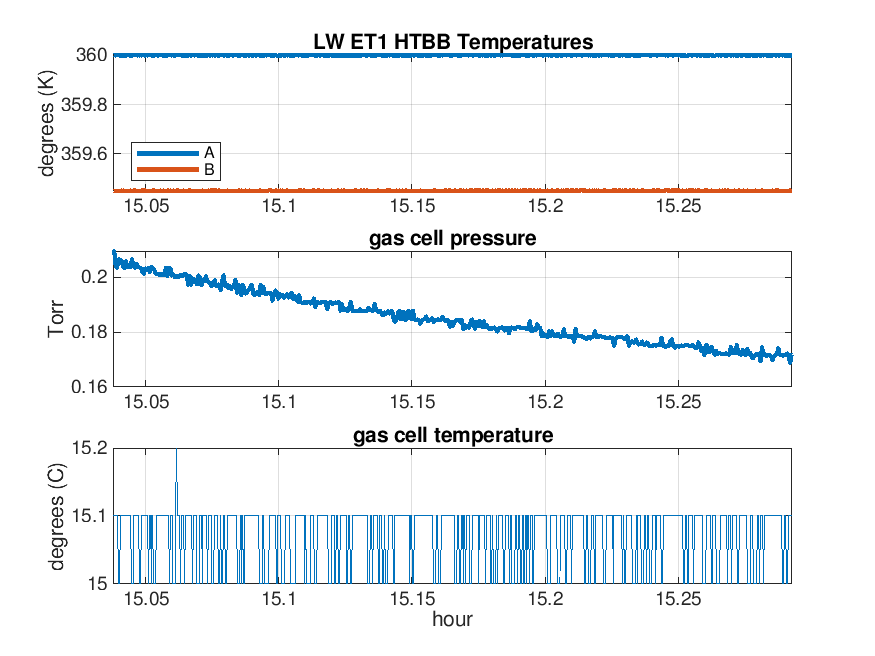
\includegraphics[width=\textwidth]{harvest_01-07/01-07_LW_ET1.png}
  \end{centering}\vspace{3mm}

  ET1 ``empty high'' leg of the the 7 Jan CO$_2$ transmittance test.
  The x-axis is hour of the day. The HTBB temps are stable but we
  see a vestigal pressure drift.

\end{column}
\begin{column}{0.5\textwidth}  
  \begin{centering}
  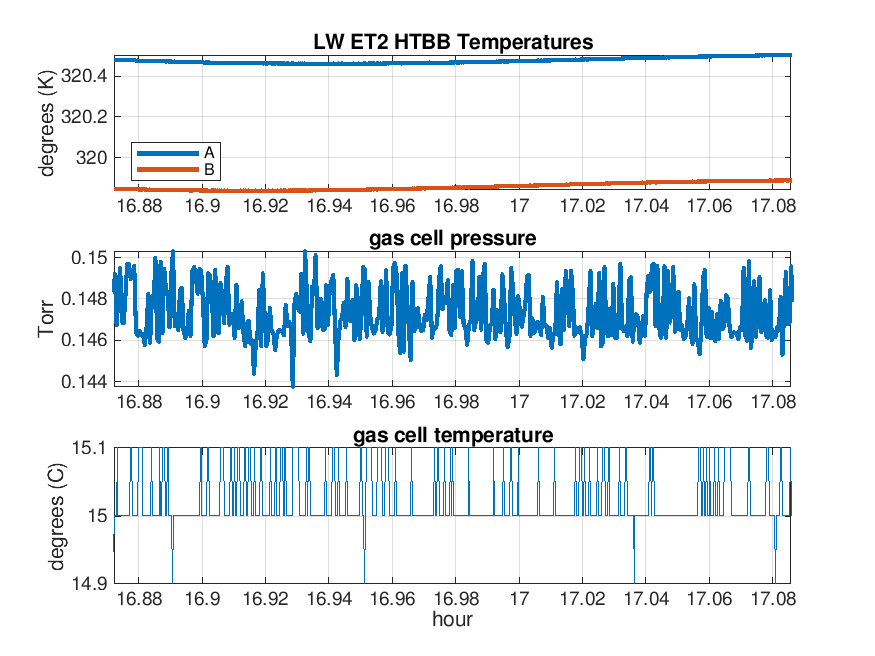
\includegraphics[width=\textwidth]{harvest_01-07/01-07_LW_ET2.png}
  \end{centering}\vspace{3mm}

  ET2 ``empty low'' leg of the the 7 Jan CO$_2$ transmittance test.
  We see a small HTBB drift.

\end{column}
\end{columns}
\end{frame}
%----------- slide --------------------------------------------------%
\begin{frame}
\frametitle{CO$_2$ PFL side 1 cell full test legs}
\begin{columns}[t]
\begin{column}{0.5\textwidth}
  \begin{centering}
  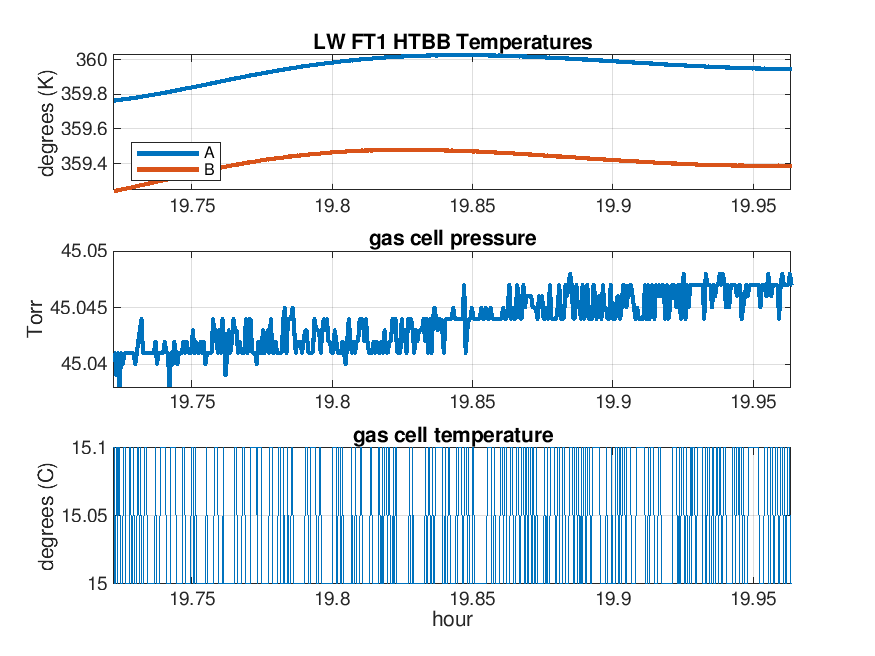
\includegraphics[width=\textwidth]{harvest_01-07/01-07_LW_FT1.png}
  \end{centering}\vspace{3mm}

  FT1 ``full high'' leg of the the 7 Jan CO$_2$ transmittance test.
  The x-axis is hour of the day.  There is significant HTBB drift.

\end{column}
\begin{column}{0.5\textwidth}  
  \begin{centering}
  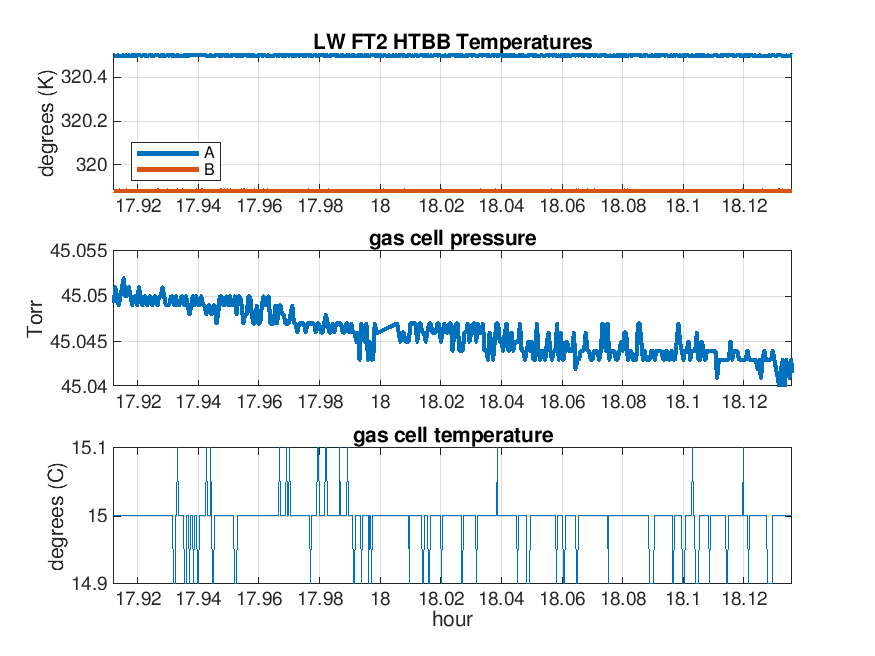
\includegraphics[width=\textwidth]{harvest_01-07/01-07_LW_FT2.png}
  \end{centering}\vspace{3mm}

  FT2 ``full low'' leg of the the 7 Jan CO$_2$ transmittance test.
  This looks good.

\end{column}
\end{columns}
\end{frame}
%----------- slide --------------------------------------------------%
\begin{frame}
\frametitle{CO$_2$ side 1 data before fitting}
\begin{columns}[t]
\begin{column}{0.5\textwidth}  
  \begin{centering}
  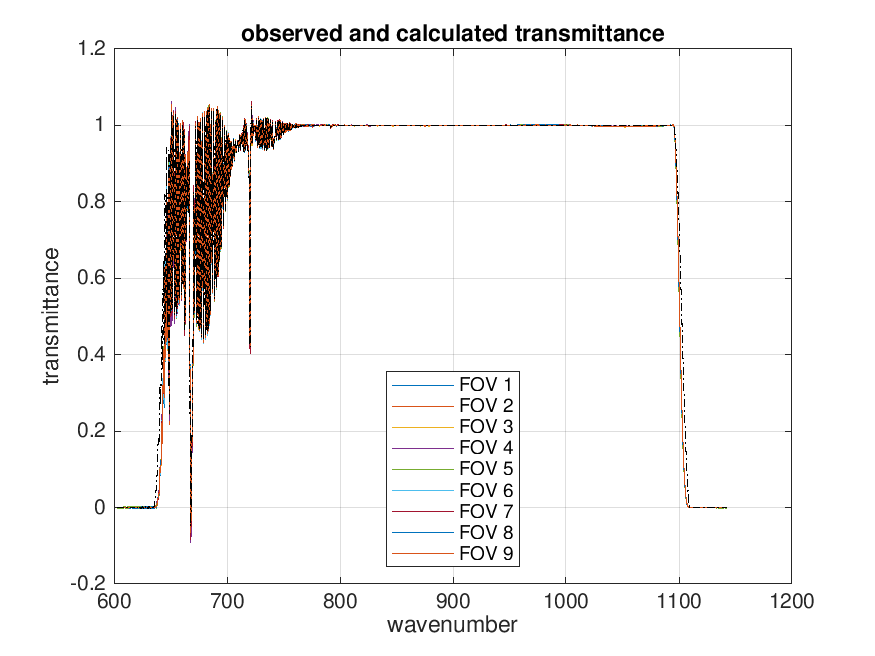
\includegraphics[width=\textwidth]{01-07_pfl_s1_CO2/spec_test2_all.png}
  \end{centering}\vspace{3mm}

Observed and calculated transmittance after the SA correction but
before any fitting.  This looks good, at this level of detail.

\end{column}

\begin{column}{0.5\textwidth}
  \begin{centering}
  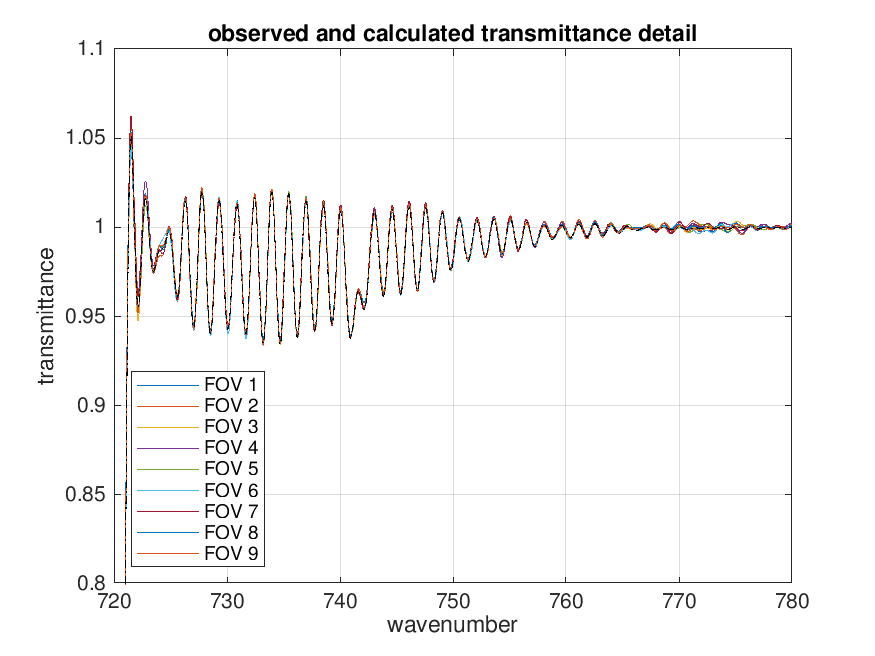
\includegraphics[width=\textwidth]{01-07_pfl_s1_CO2/spec_test2_zoom.png}
  \end{centering}\vspace{3mm}

A detail from the previous plot.  FOV to FOV consistency and
agreement with calculated transmittance is relatively good.

\end{column}
\end{columns}
\end{frame}
%----------- slide --------------------------------------------------%
\begin{frame}
\frametitle{CO$_2$ side 1 fitting overview}
\begin{columns}[t]
\begin{column}{0.5\textwidth}  
  \begin{centering}
  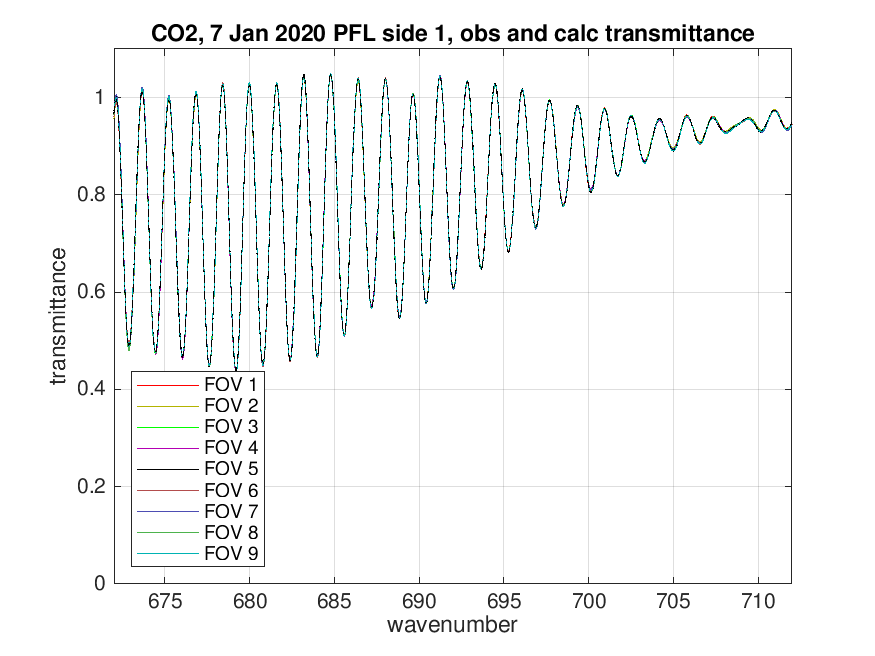
\includegraphics[width=\textwidth]{01-07_pfl_s1_CO2/CO2_obs_and_calc.png}
  \end{centering}\vspace{3mm}

Observed and calculated transmittance for all FOVs, over the fitting
interval.  At this level of detail we see all values are very close.

\end{column}

\begin{column}{0.5\textwidth}
  \begin{centering}
  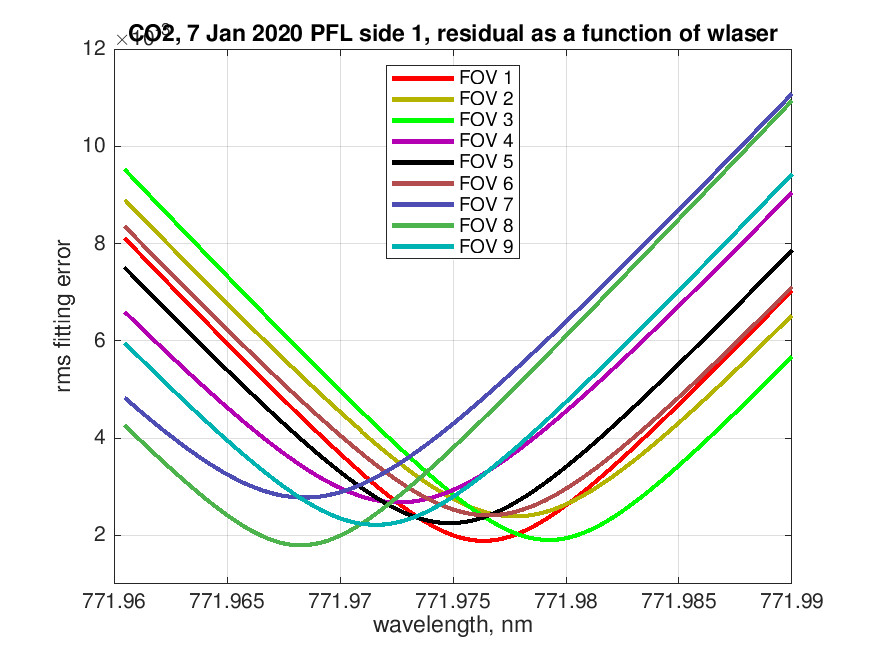
\includegraphics[width=\textwidth]{01-07_pfl_s1_CO2/CO2_wlaser_fit.png}
  \end{centering}\vspace{3mm}

Residuals $\rms(a\cdot\tauobs + b - \taucal)$ over the fitting
interval as a function of metrology laser wavelength, for each FOV.

\end{column}
\end{columns}
\end{frame}
%----------- slide --------------------------------------------------%
\begin{frame}
\frametitle{CO$_2$ side 1 obs minus calc breakouts}
\begin{columns}[t]
\begin{column}{0.5\textwidth}
  \begin{centering}
  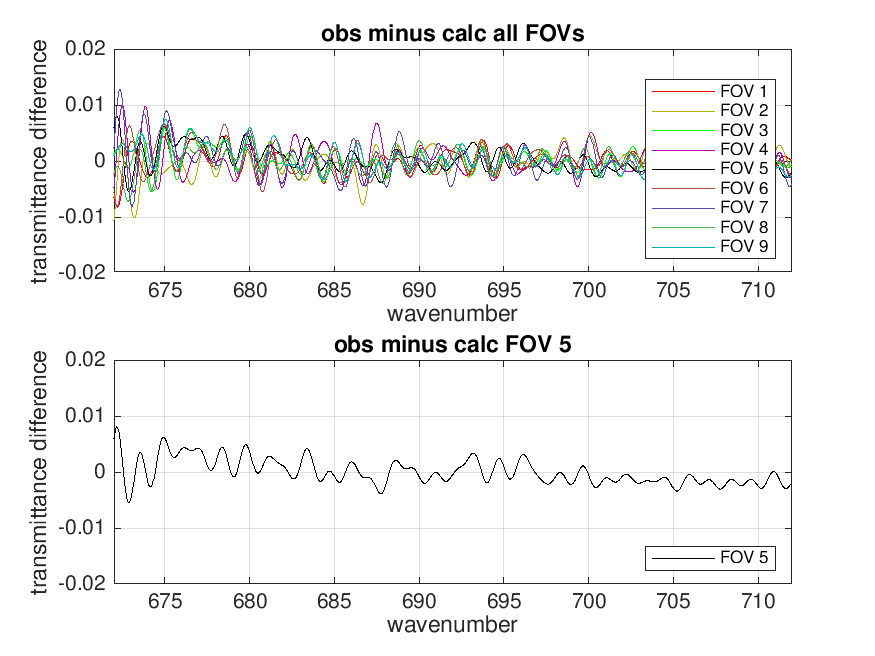
\includegraphics[width=\textwidth]{01-07_pfl_s1_CO2/CO2_breakout_1.png}
  \end{centering}\vspace{3mm}

Observed minus calculated transmittance for all FOVs and for FOV~5
alone, over the fitting interval.

\end{column}
\begin{column}{0.5\textwidth}  
  \begin{centering}
  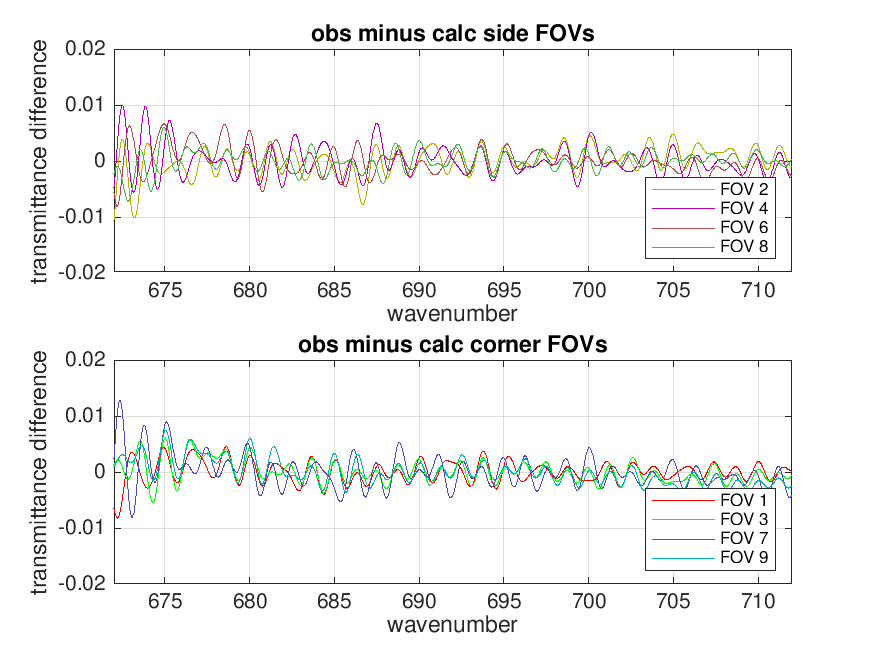
\includegraphics[width=\textwidth]{01-07_pfl_s1_CO2/CO2_breakout_2.png}
  \end{centering}\vspace{3mm}

Observed minus calculated transmittance for side and corner FOVs,
over the fitting interval.

\end{column}
\end{columns}
\end{frame}
%----------- slide --------------------------------------------------%
\begin{frame}[fragile]
\frametitle{CO$_2$ side 1 tabulated residuals}

  metrology laser absolute residuals, ppm
\begin{semiverbatim}\scriptsize
     -2.59     2.85     7.51         7   4   1
     -2.85     5.70     9.46         8   5   2
      1.42     7.90    11.40         9   6   3
\end{semiverbatim}

  metrology laser relative residuals, ppm
\begin{semiverbatim}\scriptsize
     -8.29    -2.85     1.81         7   4   1
     -8.55     0.00     3.76         8   5   2
     -4.27     2.20     5.70         9   6   3
\end{semiverbatim}

     regression fitting weights and residuals
\begin{semiverbatim}\scriptsize
 FOV   "a"       "b"     dmin     wmin      wfov
  1   0.992    0.0065   0.0019     7.51   771.9763 
  2   1.002   -0.0011   0.0024     9.46   771.9778 
  3   0.985    0.0128   0.0019    11.40   771.9793 
  4   0.991    0.0061   0.0027     2.85   771.9727 
  5   0.980    0.0171   0.0023     5.70   771.9749 
  6   0.985    0.0131   0.0024     7.90   771.9766 
  7   0.990    0.0064   0.0028    -2.59   771.9685 
  8   0.999    0.0001   0.0018    -2.85   771.9683 
  9   0.984    0.0119   0.0022     1.42   771.9716 
\end{semiverbatim}

\end{frame}
%----------- slide --------------------------------------------------%
\begin{frame}
\frametitle{CO PFL side 1 SW test parameters}

\begin{itemize}
  \item PFL Plateau 20, 8 Jan 2019
  \item side 1, sweep direction 0
  \item fitting interval 2160 to 2240 $\wn$
  \item metrology laser 771.97050 nm, from neon 703.44765 nm
  \item ATBD default focal plane
  \item SA correction from ILS with periodic sinc at the sensor grid
  \item HTBB nominal T1 335 K, T2 320 K
  \item gas cell pressure 45.92 torr
  \item gas cell temperature 14.85 C
  \item gas cell length 12.59 cm
\end{itemize}

\end{frame}
%----------- slide --------------------------------------------------%
\begin{frame}
\frametitle{CO PFL side 1 cell empty test legs}
\begin{columns}[t]
\begin{column}{0.5\textwidth}
  \begin{centering}
  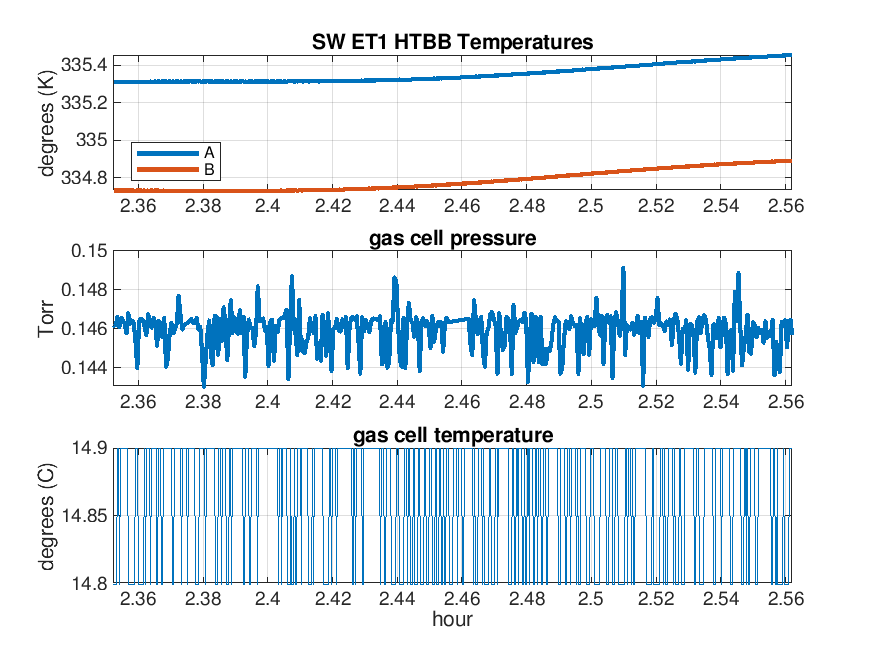
\includegraphics[width=\textwidth]{harvest_01-07/01-08_SW_ET1.png}
  \end{centering}\vspace{3mm}

  ET1 ``empty high'' leg of the the 8 Jan CO transmittance test.
  The x-axis is hour of the day.  We see some HTBB drift.

\end{column}
\begin{column}{0.5\textwidth}  
  \begin{centering}
  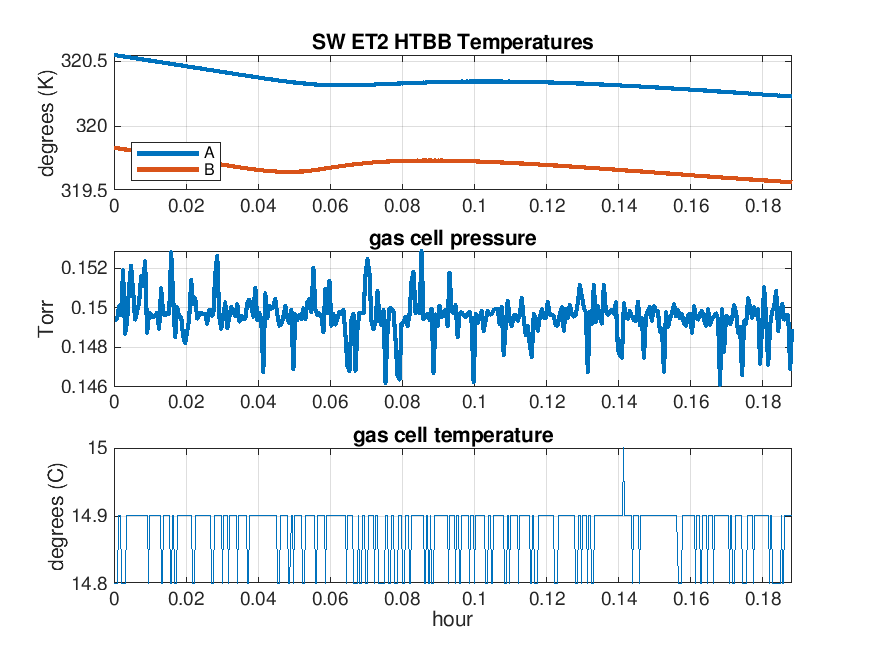
\includegraphics[width=\textwidth]{harvest_01-07/01-08_SW_ET2.png}
  \end{centering}\vspace{3mm}

  ET2 ``empty low'' leg of the the 8 Jan CO transmittance test.
  We see a significant HTBB drift.

\end{column}
\end{columns}
\end{frame}
%----------- slide --------------------------------------------------%
\begin{frame}
\frametitle{CO PFL side 1 cell full test legs}
\begin{columns}[t]
\begin{column}{0.5\textwidth}
  \begin{centering}
  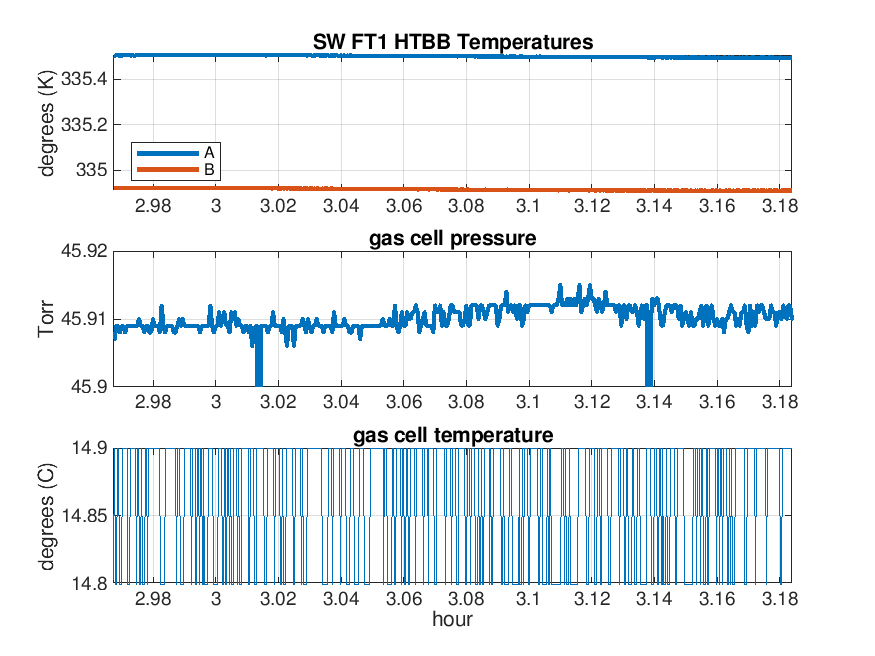
\includegraphics[width=\textwidth]{harvest_01-07/01-08_SW_FT1.png}
  \end{centering}\vspace{3mm}

  FT1 ``full high'' leg of the the 8 Jan CO transmittance test.
  The x-axis is hour of the day.  This looks good.

\end{column}
\begin{column}{0.5\textwidth}  
  \begin{centering}
  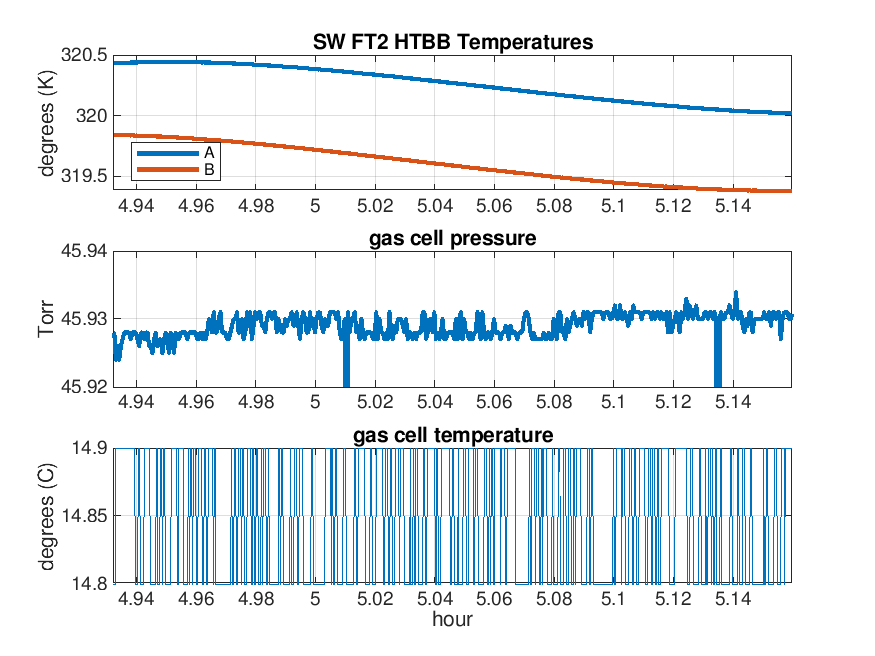
\includegraphics[width=\textwidth]{harvest_01-07/01-08_SW_FT2.png}
  \end{centering}\vspace{3mm}

  FT2 ``full low'' leg of the the 8 Jan CO transmittance test.
  There is significant HTBB drift.

\end{column}
\end{columns}
\end{frame}
%----------- slide --------------------------------------------------%
\begin{frame}
\frametitle{CO side 1 data before fitting}
\begin{columns}[t]
\begin{column}{0.5\textwidth}  
  \begin{centering}
  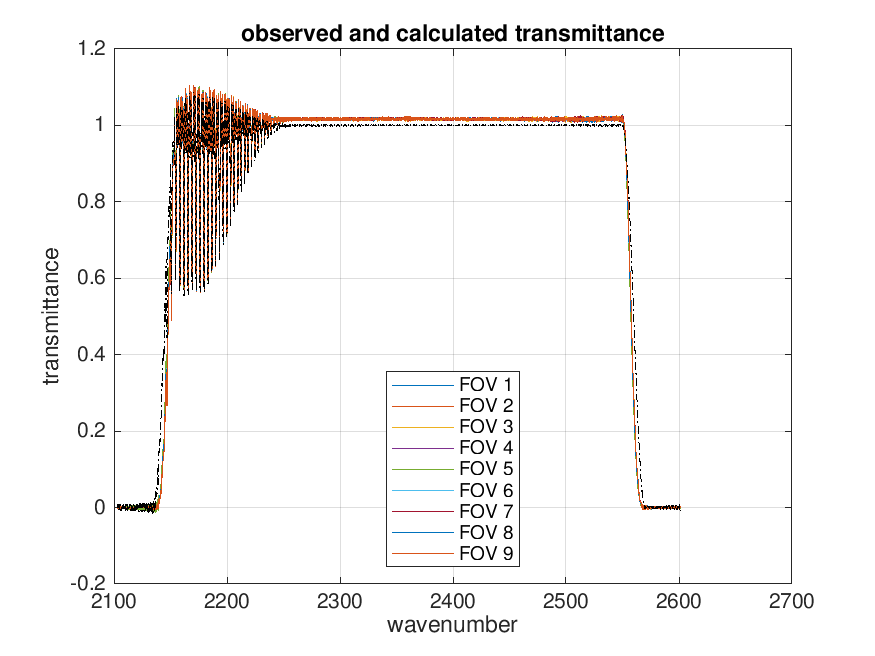
\includegraphics[width=\textwidth]{01-08_pfl_s1_CO/spec_test2_all.png}
  \end{centering}\vspace{3mm}

Observed and calculated transmittance after the SA correction but
before fitting. \\ We see some bias in the obs.

\end{column}

\begin{column}{0.5\textwidth}
  \begin{centering}
  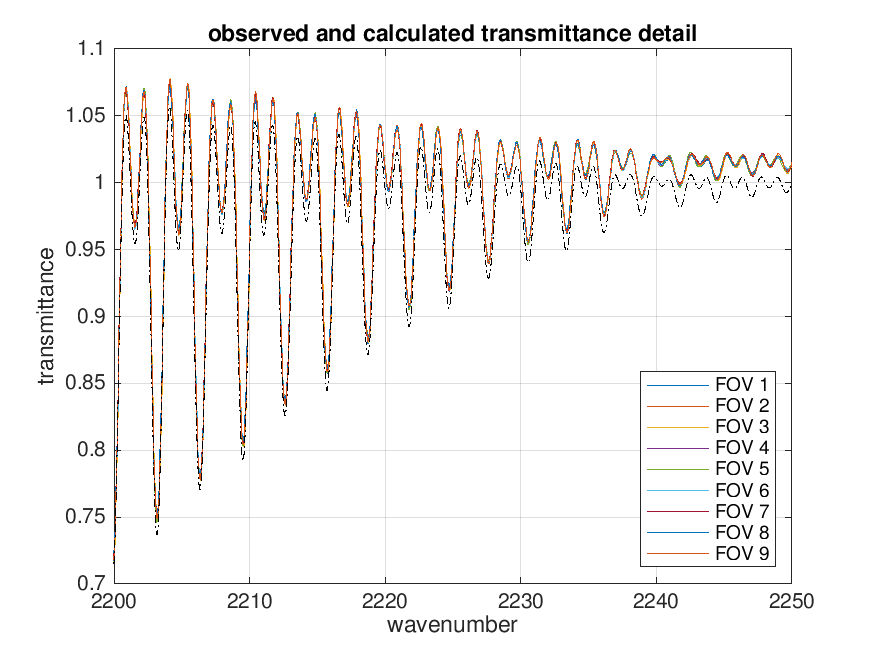
\includegraphics[width=\textwidth]{01-08_pfl_s1_CO/spec_test2_zoom.png}
  \end{centering}\vspace{3mm}

A detail from the previous plot.  Although we see some bias in the
obs, the FOV to FOV consistency is relatively good.

\end{column}
\end{columns}
\end{frame}
%----------- slide --------------------------------------------------%
\begin{frame}
\frametitle{CO side 1 fitting overview}
\begin{columns}[t]
\begin{column}{0.5\textwidth}  
  \begin{centering}
  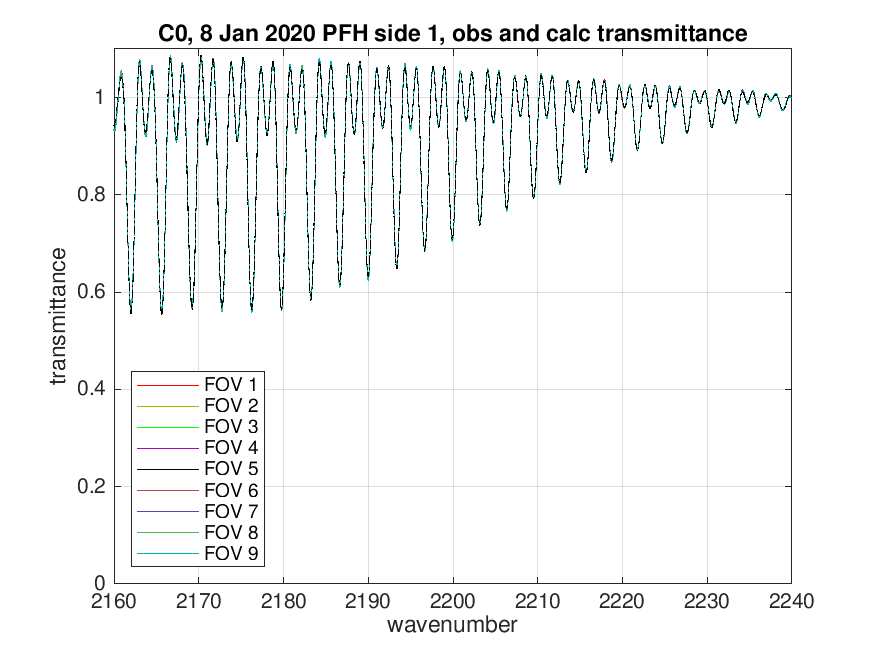
\includegraphics[width=\textwidth]{01-08_pfl_s1_CO/CO_obs_and_calc.png}
  \end{centering}\vspace{3mm}

Observed and calculated transmittance for all FOVs, over the fitting
interval.  At this level of detail we see all values are very close.

\end{column}

\begin{column}{0.5\textwidth}
  \begin{centering}
  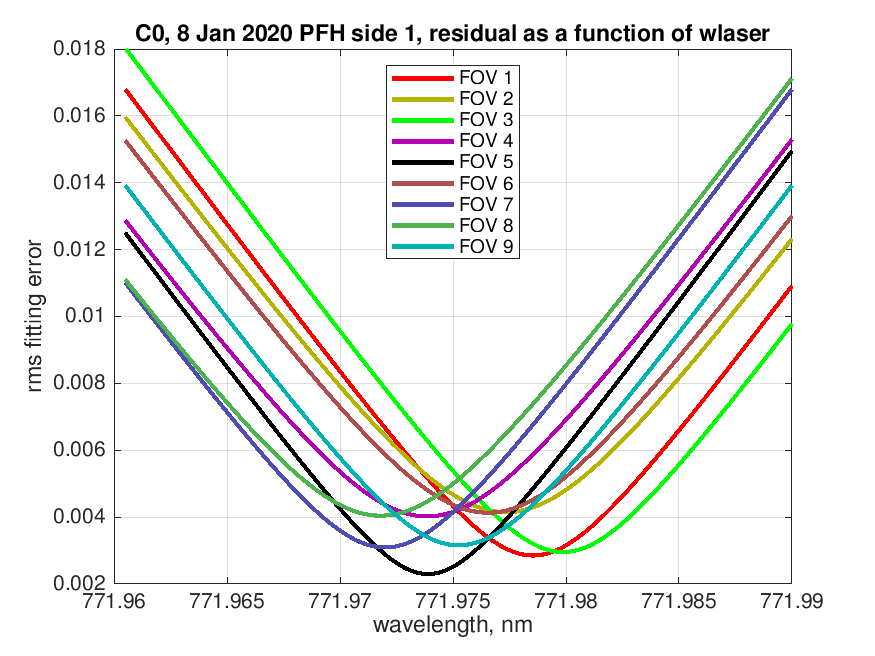
\includegraphics[width=\textwidth]{01-08_pfl_s1_CO/CO_wlaser_fit.png}
  \end{centering}\vspace{3mm}

Residuals $\rms(a\cdot\tauobs + b - \taucal)$ over the fitting
interval as a function of metrology laser wavelength, for each FOV.

\end{column}
\end{columns}
\end{frame}
%----------- slide --------------------------------------------------%
\begin{frame}
\frametitle{CO side 1 obs minus calc breakouts}
\begin{columns}[t]
\begin{column}{0.5\textwidth}
  \begin{centering}
  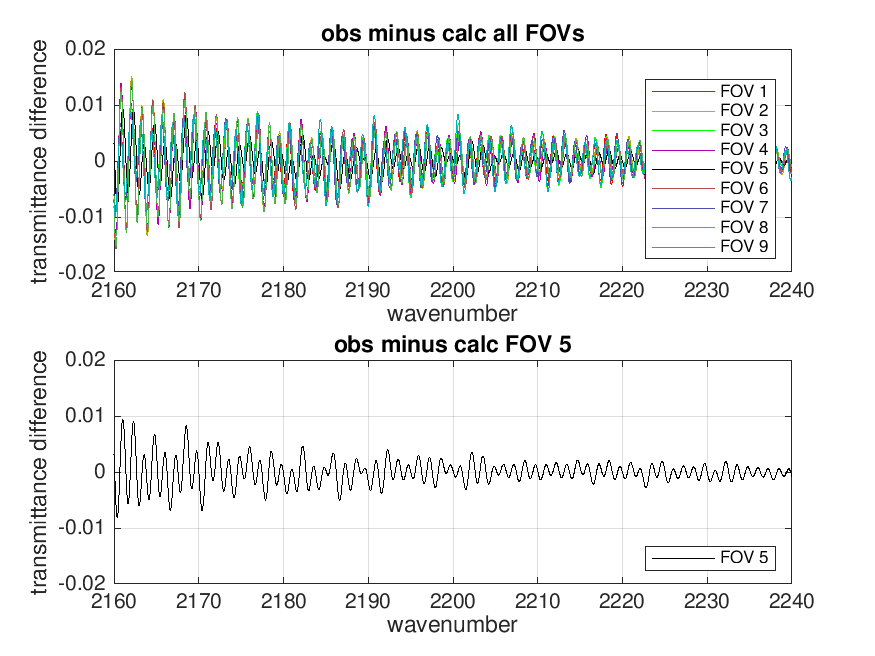
\includegraphics[width=\textwidth]{01-08_pfl_s1_CO/CO_breakout_1.png}
  \end{centering}\vspace{3mm}

Observed minus calculated transmittance for all FOVs and for FOV~5
alone, over the fitting interval.

\end{column}
\begin{column}{0.5\textwidth}  
  \begin{centering}
  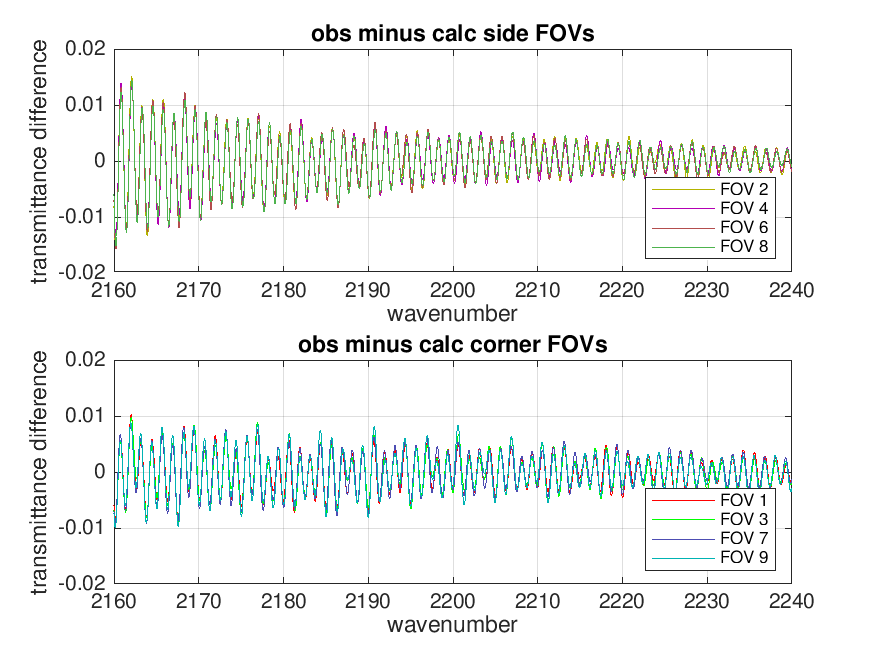
\includegraphics[width=\textwidth]{01-08_pfl_s1_CO/CO_breakout_2.png}
  \end{centering}\vspace{3mm}

Observed minus calculated transmittance for side and corner FOVs,
over the fitting interval.

\end{column}
\end{columns}
\end{frame}
%----------- slide --------------------------------------------------%
\begin{frame}[fragile]
\frametitle{CO side 1 tabulated residuals}

  metrology laser absolute residuals, ppm
\begin{semiverbatim}\scriptsize
      1.94     4.40    10.36         7   4   1
      1.68     4.40     8.81         8   5   2
      6.22     7.77    12.18         9   6   3
\end{semiverbatim}

  metrology laser relative residuals, ppm
\begin{semiverbatim}\scriptsize
     -2.46     0.00     5.96         7   4   1
     -2.72     0.00     4.40         8   5   2
      1.81     3.37     7.77         9   6   3
\end{semiverbatim}

     regression fitting weights and residuals
\begin{semiverbatim}\scriptsize
 FOV   "a"       "b"     dmin     wmin      wfov
  1   0.972    0.0128   0.0029    10.36   771.9785 
  2   0.976    0.0088   0.0041     8.81   771.9773 
  3   0.973    0.0116   0.0030    12.18   771.9799 
  4   0.980    0.0044   0.0040     4.40   771.9739 
  5   0.973    0.0107   0.0023     4.40   771.9739 
  6   0.979    0.0056   0.0041     7.77   771.9765 
  7   0.978    0.0059   0.0031     1.94   771.9720 
  8   0.981    0.0027   0.0040     1.68   771.9718 
  9   0.972    0.0118   0.0032     6.22   771.9753 
\end{semiverbatim}

\end{frame}
%----------- slide --------------------------------------------------%
\begin{frame}
\frametitle{Conclusions}
\begin{itemize}

  \item We have done a preliminary analysis of the PFL Plateau 20
    CH$_4$, CO$_2$, and CO gas cell tests, and compared these with
    calculated reference truth.  Overall, the results look quite
    good.

  \item The HTBB drift seen in many of the test legs is significant
    but managable with our approach to regression fitting.   The effect
    of the drifts could be reduced with more careful subsetting, if
    needed.

  \item Metrology laser relative residuals are in reasonable
    agreement, and can be reduced further with focal plane
    adjustments.  Metrology laser absolute residuals could be
    reduced with a more judicious choice of neon wavelengh, or 
    possibly by simply using the eng neon value.

\end{itemize}
\end{frame}
%----------- slide --------------------------------------------------%

\end{document}

